\documentclass[preview]{standalone}

\usepackage[english]{babel}
\usepackage{amsmath}
\usepackage{amssymb}

\usepackage{tikz}
\usetikzlibrary{arrows}
\begin{document}

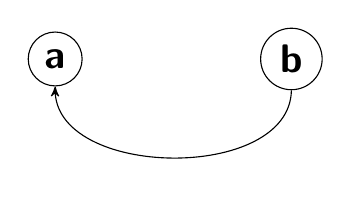
\begin{tikzpicture}
[->,>=stealth',node distance=3cm]
            \node[circle,draw=black,font=\sffamily\Large\bfseries] (1) {\textcolor{black}{a}};
            \node[circle,draw=black,text=black,font=\sffamily\Large\bfseries] (2) [right of=1] {b};
            \path[every node/.style={color=green,font=\sffamily\small}] (2) edge[bend left=90] node [left] {} (1);
\end{tikzpicture}

\end{document}
